\chapter{System Design}\label{chap:design}
% \section{Teat Pose Estimation System Design}
\label{Background}
% 3-6 pages
\lipsum[1]\todo{TODO}

In the following sections we describe the architecture of the components required for estimating the cow teat poses. These components execute an essential role in processing pipelines which process the camera information published, identify salient objects and finally estimate the cow teat pose. We also set out the assumptions we took and the choices of technologies with respect to what was discussed in Section 2.

% domain model
%  
\section{FMC Diagram}
The Fundamental Modeling Concepts (FMC) provide a framework for the comprehensive description of software-intensive systems. 
% Its block diagrams show the compositional structures as a composition of collaborating system components.
Active system components are called agents and passive system components are called locations (storage, channels, queues; where information can be observed) \cite{FMCdiag}. The following FMC diagram (Figure \ref{fig:cow_fmc}) describes the high-level overview of the system's architecture.
    \begin{figure}[!ht]
        \centering
        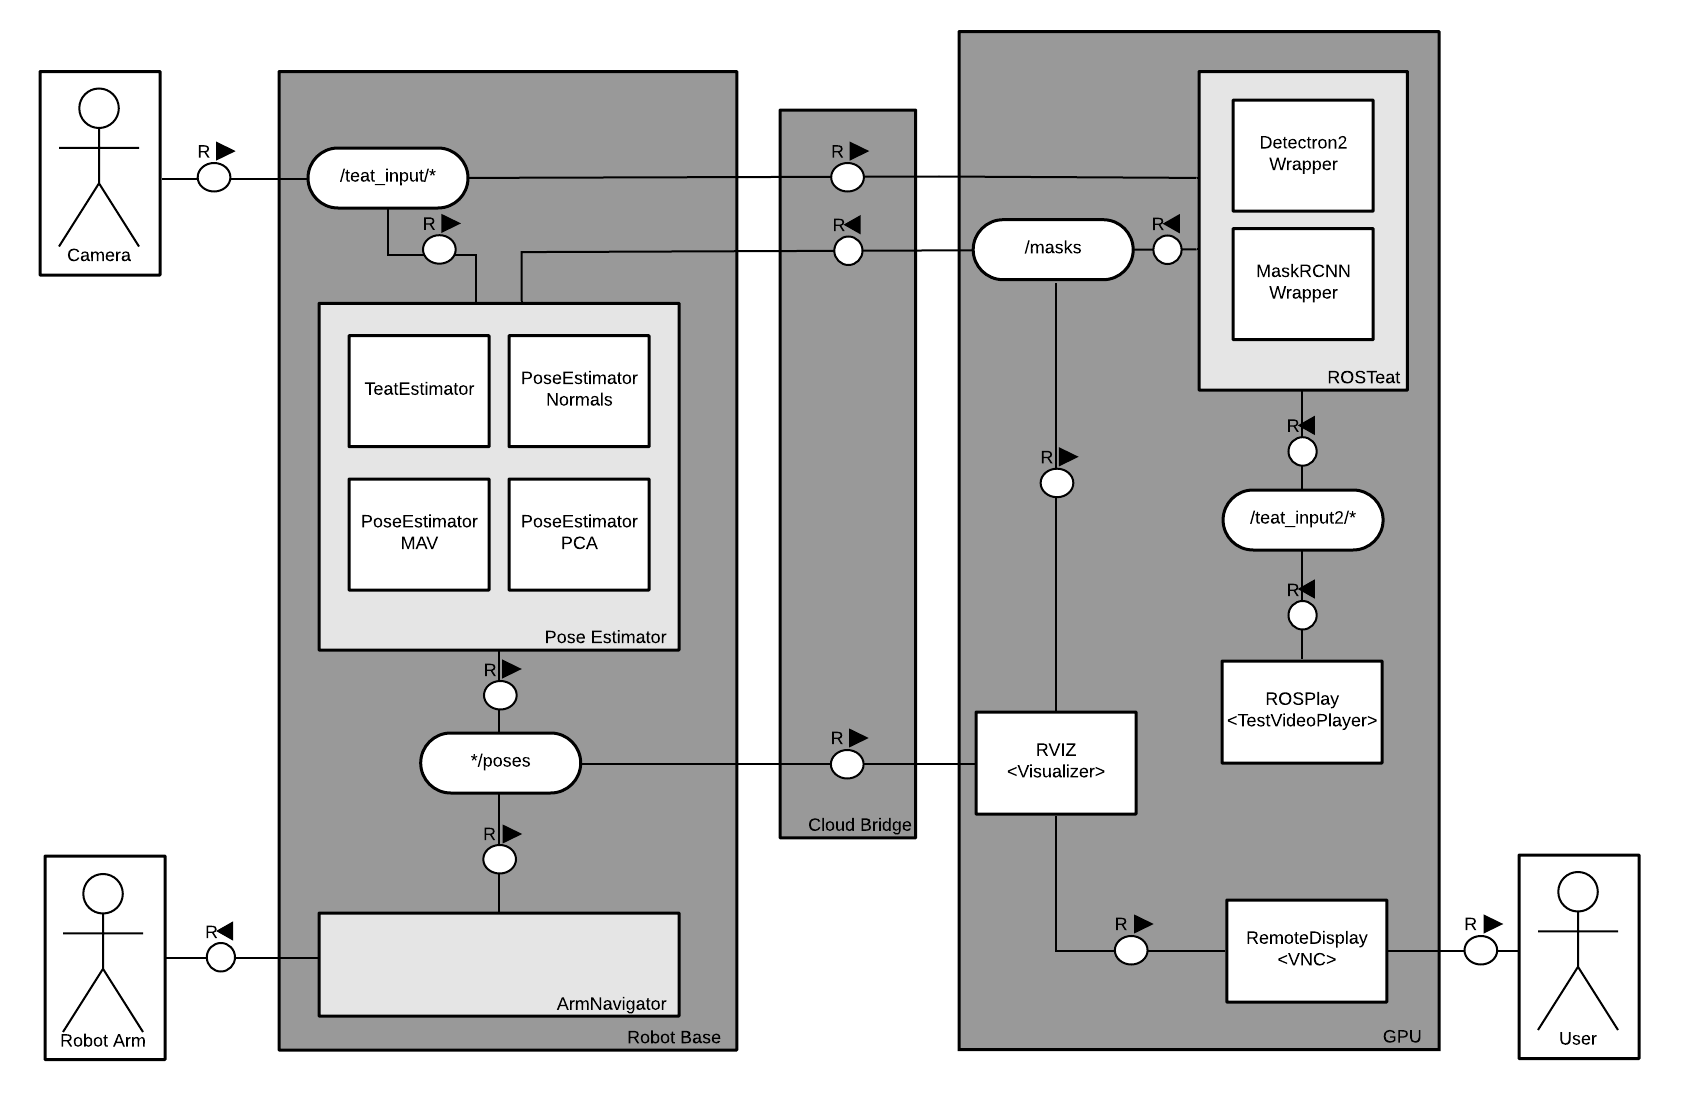
\includegraphics[width=1\textwidth]{images/cow_fmc.png}
        \caption{A prototype of the Job Information dialog}
        \label{fig:cow_fmc}
    \end{figure}
    
% \newpage
\lipsum[2]\todo{TODO}
The FMC diagram in Figure \ref{fig:cow_fmc} describes the following agents and locations:
\begin{itemize}
    \item \textbf{Camera:} captures frames and publishes these as input for all the other components.
    \item \textbf{User:} uses Rviz to visualize: the point cloud, the RGB image, the depth image, the segmented image of the cow teats and the 3D poses published.
    \item \textbf{Robot Arm:} moves according to the instructions given by ArmNavigator. 
    \item \textbf{PoseEstimator:} pose estimation algorithm that processes the information received from the camera and ROSTeat to predict 3D poses.
    \item \textbf{ROSTeat Node:} processes images from the Camera node and segments the cow teats in the image.
    \item \textbf{ArmNavigator:} manipulates the RobotArm according to the 3D poses published.
    \item \textbf{ROSPlay <TestVideoPlayer> Node:} Behaves as a simulation/testing mechanism for reproducing the camera videos.
    \item \textbf{RVIZ <Visualizer>:} ROS framework that allows the visualization of different ROS topics (RGB image, point cloud, etc.)
    \item \textbf{RemoteDisplay <VNC>:} this is a browser-based graphical-d
    esktop system that allows the visualization of RVIZ.
    \item \textbf{/teat input/*:} channel where the camera input is published for other components to consume.
    \item \textbf{/teat input2/*:} channel where the simulation video is published as input for other components to consume.
    \item \textbf{/masks:} channel where the segmented cow teats are published.
    \item \textbf{*/poses:} channel wehre the 3D cow teat poses are published.
\end{itemize}

The behavior and interactions of the main components (ROSTeat and Pose Estimator) are described in the following sections with more detail.

\section{Use Cases}
\lipsum[2]\todo{TODO}
\begin{longtable}{@{} p{3.5cm} p{10.5cm} @{}} \toprule
\textbf{Use Case}       & \textbf{Predict Cow Teat Masks} \\ \midrule
Actor                   & ROSTeat Node \\ \cmidrule{1-2}
Description             & A cow teat is recognized from an image. \\ \cmidrule{1-2}
Goal                    & Publish the cow teat masks present in received image. \\ \cmidrule{1-2}
Preconditions           & An image exists. \\ 
                        & ROSTeat node is running. \\ \cmidrule{1-2} 
Postconditions          & A number of masks have been identified from image [0+]\\ \cmidrule{1-2} 
                        & 1. The camera publishes an image. \\ 
Basic Flow              & 2. The ROSTeat node consumes the image and predicts the cow teats in it. \\
                        & 3. The ROSTeat node publishes the masks for future processing. \\ \cmidrule{1-2}
Exceptions             & Image is not RGB \\ \bottomrule
\caption{Use Case - Predict Masks} \label{tab:tabcu-prop} \\
\end{longtable}

% \newpage
\begin{longtable}{@{} p{3.5cm} p{10.5cm} @{}} \toprule
\textbf{Use Case}       & \textbf{Estimate Cow Teat Pose} \\ \midrule
Actor                   & Pose Estimator \\ \cmidrule{1-2}
Description             & A cow teat pose is recognized from a tuple (image, point cloud, depth image, mask). \\ \cmidrule{1-2}
Goal                    & Publish the cow teat poses for each message received. \\ \cmidrule{1-2}
Preconditions           & An image exists. \\ 
                        & ROSTeat node is running. \\ \cmidrule{1-2} 
Postconditions          & A number of cow teat poses have been identified from image [0+]\\ \cmidrule{1-2} 
                        & 1. The camera publishes an image AND ROSTeat node publishes the masks for the image (synchronized receival, stored as a tuple). \\ 
Basic Flow              & 2. The Pose Estimator node consumes the tuple and predicts the cow teat poses in it. \\
                        & 3. The Pose Estimator node publishes the poses for posterior attachment. \\ \cmidrule{1-2}
Exceptions             & TransformListener is empty \\ 
                       & Any element in the tuple is empty and masks are not (data corruption). \\ \bottomrule
\caption{Use Case - Predict Poses} \label{tab:tabcu-prop} \\
\end{longtable}
\lipsum[2]\todo{TODO}

\section{Processing Pipeline}
    The deployment of the components was done using docker compose files to leverage the capabilities of microservices, where every component used behaves as a separate component in the application. The benefit gotten out of microservices is that they are small in size, bounded by their context, independently developed and deployable and they allow for message-based communication%todo ADD REF
    . 
    
    The set of libraries and tools used for building the robot application for pose estimation was the Robot Operating System (ROS)%todo ADD REF
    . ROS uses 'topics' as named buses over which ROS nodes exchange messages\ref{ros:topics}. %http://wiki.ros.org/Topics
    Figure \ref{fig:cow_topics} shows a high-level overview of the communication fashion between components, where the messages go through a ROS Cloud Bridge to be able to connect the robot's ROS local topics with the GPU ROS topics. 
  
    
    The architecture of the pipeline was designed so that the interfaces between components would be standarized in the topics message communication. Therefore, any teat points extraction algorithm could be used to consume the camera information and predict a 3D pose. The pipeline's design is described below:
    \begin{enumerate}
        \item The camera publishes information (RGB image, point cloud, depth image) into the input ROS topic channel, which is consumed to identify the position and size of salient objects.
        \item The ROSTeat node subscribes to this input channel, uses the neural network to predict the cow teat masks and publishes them into a masks channel.
        \item The Pose Estimator (plug-and-play component) consumes the masks that were published, and synchronizes it with the camera information (so it is all processed as a single message). The following pose estimation is algorithm-specific. Each pose estimation algorithm is described in detail in the following section. The poses are then published into a poses channel.
        \item The robot consumes messages from the poses channel and moves 10-15 cm forward towards the indicated 3D poses, until it is 20-30 cm close to the pose estimations. Then the attachment process is initiated.
    \end{enumerate}
    \begin{figure}[!ht]
        \centering
        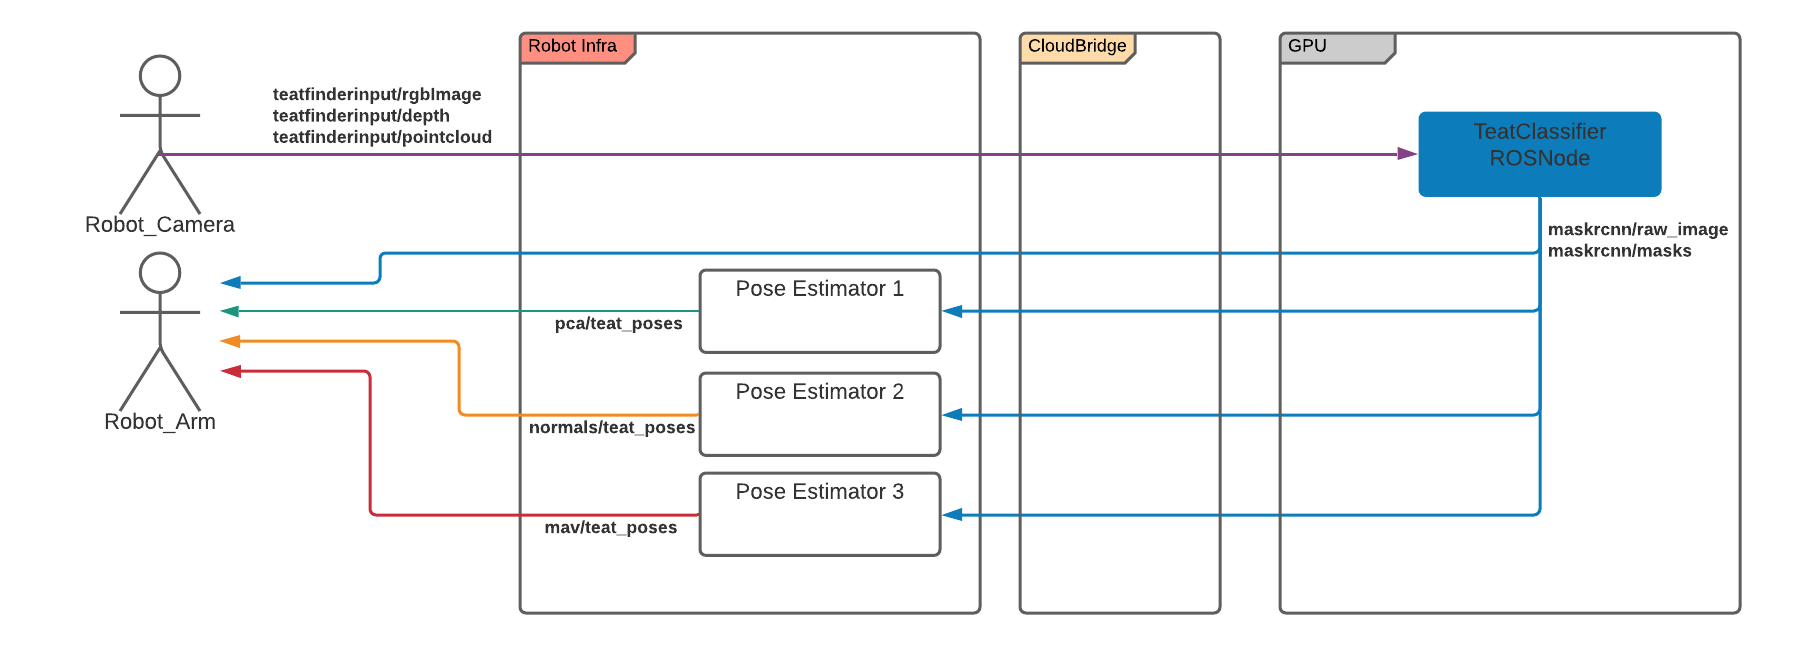
\includegraphics[width=1\textwidth]{images/cow_topics.png}
        \caption{A prototype of the Job Information dialog}
        \label{fig:cow_topics}
    \end{figure}
    
    \lipsum[2]\todo{TODO}. The described pipeline can also be represented visually as shown by Figure \ref{fig:cow_design}.
    % The pose estimation algorithm was evaluated by error to GT
    \begin{figure}[!ht]
        \centering
        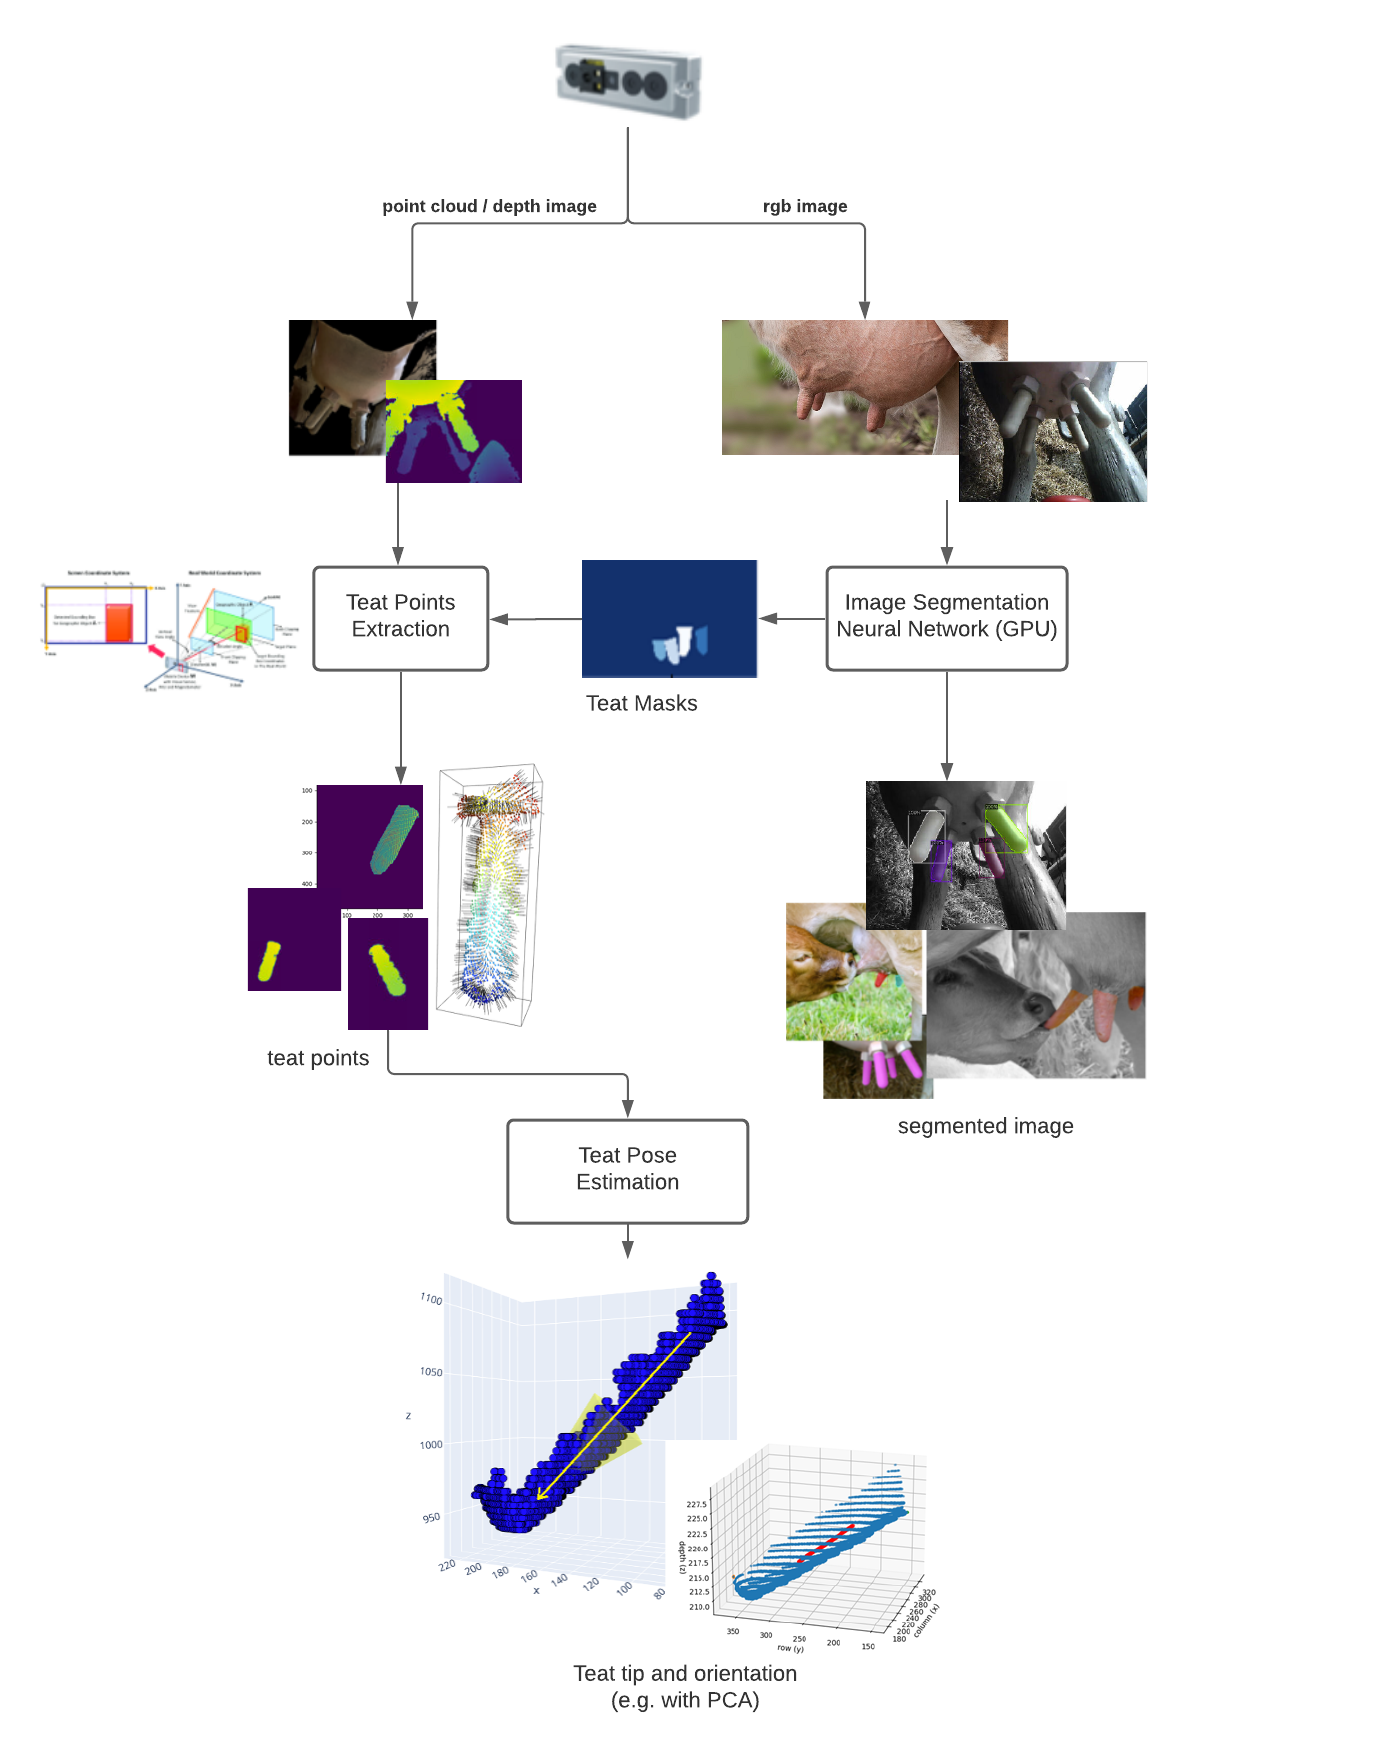
\includegraphics[width=0.9\textwidth]{images/cow_design.png}
        \caption{A prototype of the Job Information dialog}
        \label{fig:cow_design}
    \end{figure}
    
    % \begin{figure}[h]
    %     \centering
    %     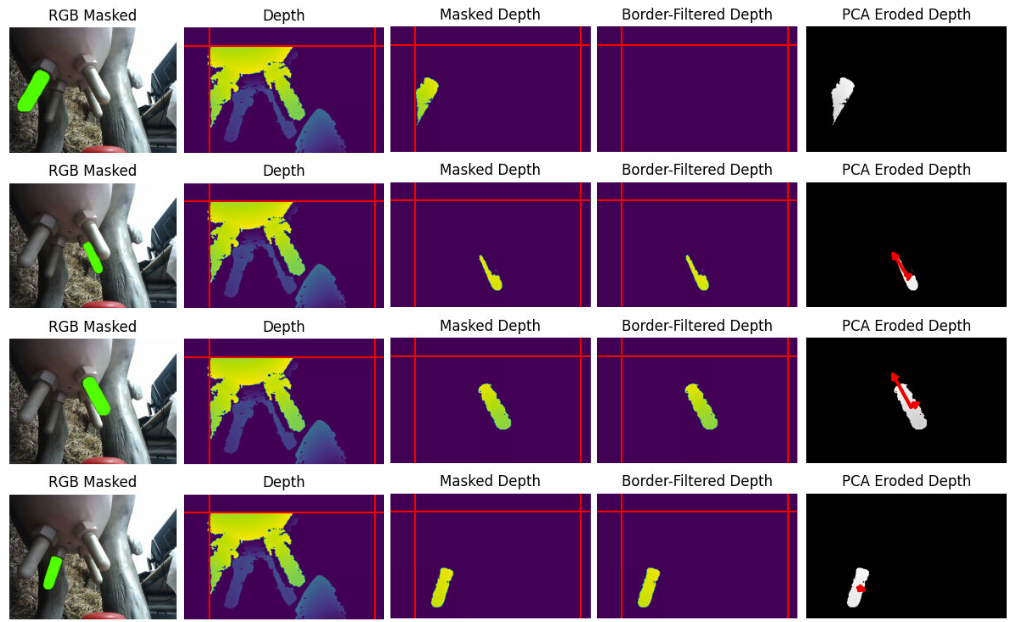
\includegraphics[width=0.6\textwidth]{images/cow_segment.png}
    %     \caption{A prototype of the Job Information dialog}
    %     \label{fig:cow_design}
    % \end{figure}
    
    % \begin{itemize}
    %     \item rgb input, setup of the cow and angle of the camera 
    %     \item networks architectures tried out: maskrcnn + pca, detectron + pca + subvariants
    % \end{itemize}

\section{Object Segmentation}
Object detection is a computer vision task that attempts to localize and classify objects within an image. An extension of the problem involves assigning labels to the specific pixels in the image that belong to the detected objects, instead of only using the bounding boxes obtained during localization (object segmentation). 

Research on object segmentation built upon previous models to reach the current state of the art of 2D object detection, which is called Mask R-CNN. The image saliency approach each (previous) model takes is described below:
\begin{itemize}
    \item \textbf{R-CNN:} a “selective search” algorithm proposes bounding boxes and features are obtained using a deep convolutional neural network (for example, AlexNet). Object classifications are then made with linear SVMs.
    \item \textbf{Fast R-CNN:} unifies the feature detector, and the bounding box predictor approach into a single model, but the region of interests are still part of the input. The shared computation showed speed improvements.
    \item \textbf{Faster R-CNN:} unifies the region proposal algorithm into the CNN model. This model merges a RPN (region proposal network) with Fast R-CNN.
    \item \textbf{Mask R-CNN:} extends the previous model to add pixel-level image segmentation. A small fully connected network was added that per region of interest outputs a segmentation mask.
\end{itemize}

The cow teat segmentation problem was tackled using two implementations of MaskRCNN: matterport/MaskRCNN and Detectron2 (FacebookAI). The evaluation and performance of both approaches is described in Section 5.

%As of 28.12.2020, MaskRCNN's repository has not been updated since 01.04.2019 and has over 1500 issues.

\section{Pose Estimation}
We rely on the RGB-D input received from the camera, where each image has a resolution of 640 x 480 x 4 pixels. Each pose estimation algorithm receives the input from the camera and the segmentation mask and processes it differently. This was done to analyze the precision from different sources of information (for example, point cloud versus depth image).

    \subsection{Point Cloud}
    
    % !TODO
    \lipsum[2-3]
    This setup consists of the following steps:\todo{TODO}
        \begin{itemize}
        \item identify first principal component V
        \item check V's explained variance ratio > 70% (i.e., the teat is "longer than wider")
        \item transform points using PCA frames
        \item find min and max points in V direction
        \item use camera pose to find out if tip is at min/max
        \end{itemize}.
    \begin{figure}[!ht]
        \centering
        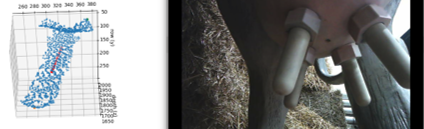
\includegraphics[width=0.8\textwidth]{images/cow_pca.png}
        \caption{A prototype of the Job Information dialog}
        \label{fig:cow_fmc}
    \end{figure}
    
    The assumptions this method makes are:
    \begin{itemize}
        \item Teats are longer than wider
        \item Tips are visible and camera angle doesn't reduce resolution in one dimension
        \item Teats point downwards
    \end{itemize}
    \lipsum[2-3]\todo{TODO}
    
    \subsection{Normals}
    

    
    
    \lipsum[2-3]
    This setup consists of the following steps:
        \begin{itemize}
        \item identify teat axis by minimizing sum of dot products of all normal vectors
        \item transform points using axis as principal component
        \item find min and max points in axis direction
        \item  camera pose to find out if tip is at min/max
        \end{itemize}.
    % \begin{wrapfigure}{r}{0.35\textwidth}
    %     \centering
    %     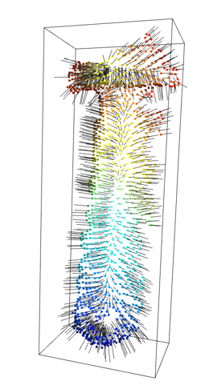
\includegraphics[width=0.2\textwidth]{images/cow_normals.png}
    %     \caption{A prototype of the Job Information dialog}
    %     \label{fig:cow_fmc}
    % \end{wrapfigure}
    
    \begin{figure}[!ht]
        \centering
        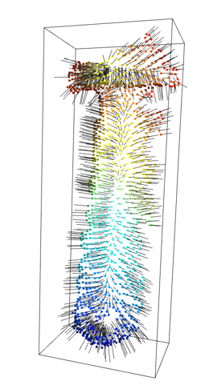
\includegraphics[width=0.2\textwidth]{images/cow_normals.png}
        \caption{A prototype of the Job Information dialog}
        \label{fig:cow_fmc}
    \end{figure}
    
    The assumptions this method makes are:
        \begin{itemize}
        \item Teat surface normals are "computable" (i.e. teat is close enough we see surface curvature)
        \item Teat is roughly cylindric in shape
        \item Tips are visible
        \item Teats point downward
        \end{itemize}
   \lipsum[2-3]\todo{TODO}

    
    \subsection{Depth Image}
    \begin{figure}[!ht]
        \centering
        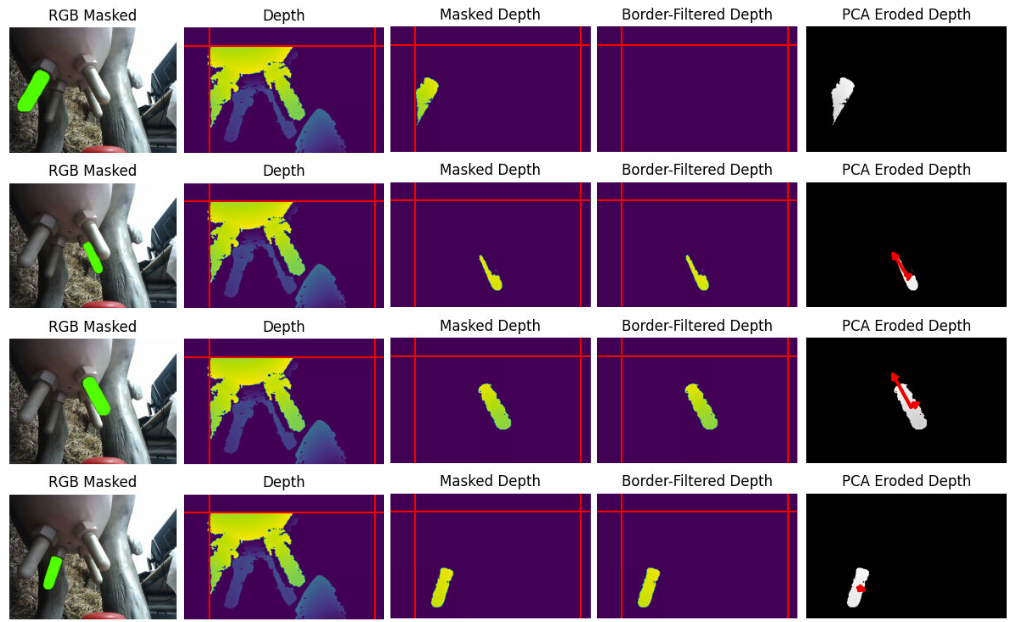
\includegraphics[width=0.7\textwidth]{images/cow_segment.png}
        \caption{A prototype of the Job Information dialog}
        \label{fig:cow_fmc}
    \end{figure}
    \lipsum[2-3]\todo{TODO}
    This setup consists of the following steps:
        \begin{itemize}
        \item RGB teat mask obtained from Detectron2
        \item Clear border-masks to avoid cut objects (rgb mask)
        \item Depth masked by the RGB mask received
        \item Clear border-masks to avoid cut objects (depth mask has different resolution)
        \item Teat width calculated from masked-depth (2D) to calculate an offset*
        \item Depth information (masked-depth) pushed to the 3D space
        \item PCA used on depth to identify teat coordinates
        \item Obtain Pose with: teat coordinates + PCA information 
        \item 4-queue structure with "memory", used to manipulate, organize and filter Poses
        \end{itemize}
    
    The assumptions this method makes are:
        \begin{itemize}
            \item Teats are longer than wider
            \item Tips are visible and camera angle doesn't reduce resolution in one dimension
            \item Teats point downward
            \item Depending on memory of queues, the algorithm can adapt quickly or slowly to new teats (timestamp filtering on the backlog)
        \end{itemize}
    \lipsum[2]\todo{TODO}
    
    While the baseline approach using just a CNN is not even in theory capable of accumulating enough
information of the scene to answer all questions posed in section 3.1, it is instead much easier to
train a neural network which does not use image sequences but independent images only as input, due
to its lower dimensionality. Each architecture setup is composed from a number of sub-networks for
better reusability. The CNN + RNN version for example uses the same feature extraction layer as the
baseline version and all three setups rely on the same number of fully connected layers for creating the
scene embedding vector. 
% The backpropagation of error is performed end-to-end through all different sub-networks. The streams that output information regarding a single object are evaluated multiple times on each timestep using randomly selected objects and their loss is accumulated. The enumerating stream which is designed to output all objects is evaluated once each frame.
The performance evaluation of these algorithms is described in Chapter \ref{chap:evaluation}.
